\documentclass[border=4pt]{standalone}
\usepackage{amsmath,amssymb,amsfonts}
\usepackage{xcolor,colortbl,array,booktabs,multirow}
\usepackage{tikz}
\usepackage{pgfplots}
\pgfplotsset{compat=1.16}
\usetikzlibrary{arrows, automata, backgrounds, calendar, chains, decorations,
    matrix, mindmap, patterns, petri, positioning, shadows, shapes.geometric,
    trees, shapes, decorations.pathreplacing, calc, tikzmark, arrows.meta,
    intersections, fit, graphs, quotes, angles, decorations.markings}
\newcommand{\st}{\text{ s.t. }}
\newcommand{\x}{\mathbf{x}}
\renewcommand{\b}{\mathbf{b}}
\renewcommand{\c}{\mathbf{c}}
\newcommand{\A}{\mathbf{A}}
\newcommand{\y}{\mathbf{y}}
\newcommand{\z}{\mathbf{z}}
\newcommand{\R}{\mathbb{R}}
\newcommand{\RR}{\mathbb{R}}
\newcommand{\Z}{\mathbb{Z}}
\newcommand{\ZZ}{\mathbb{Z}}
\newcommand{\npcomplete}{NP-complete}
\providecommand{\true}{\text{TRUE}}
\providecommand{\false}{\text{FALSE}}
\tikzset{vertex/.style={circle,fill=black!25,minimum size=20pt,inner sep=0pt},
    edge/.style={draw,thick,-},weight/.style={font=\small},
    selected vertex/.style={vertex, fill=red!24},
    selected edge/.style={draw,line width=2pt,-,red!50},
    ignored edge/.style={draw,line width=2pt,-,black!20}}
\newcommand{\vect}{\vec}
\providecommand{\ds}{\displaystyle}
\providecommand{\longvect}{\overrightarrow}
\usepackage[normalem]{ulem}
\definecolor{ocre}{RGB}{243,102,25}
\providecommand{\leftB}{\left[}
\providecommand{\rightB}{\right]}
\tikzset{directed/.style={postaction={decorate,decoration={markings,mark=at position .65 with {\arrow{>}}}}},
    directed1/.style={postaction={decorate,decoration={markings,mark=at position .65 with {\arrow{>}}}}}}
\begin{document}
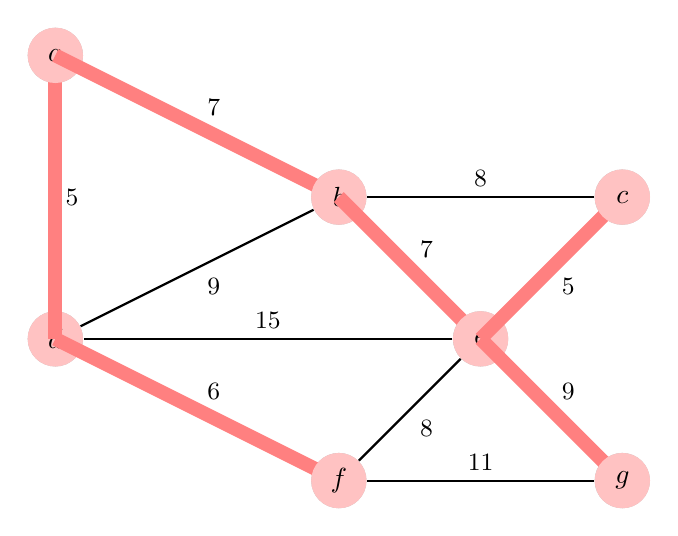
\begin{tikzpicture}[scale=1.8, auto,swap]

  % Draw a 7,11 network
  
  % First we draw the vertices
  
  \foreach \pos/\name in {{(0,2)/a}, {(2,1)/b}, {(4,1)/c},
                          {(0,0)/d}, {(3,0)/e}, {(2,-1)/f}, {(4,-1)/g}}
    \node[circle,fill=black!25,minimum size=20pt,inner sep=0pt] (\name) at \pos {$\name$};

  % Connect vertices with edges and draw weights  
  \foreach \source/ \dest / \weight in {b/a/7, c/b/8, d/a/5, d/b/9,
                                       e/b/7, e/c/5, e/d/15,
                                       f/d/6, f/e/8,
                                       g/e/9, g/f/11}
    \path[draw,thick,-] (\source) -- node[font=\small] {$\weight$} (\dest);

% solution edges

  % Vertex d
  \node[circle,fill=red!24,minimum size=20pt,inner sep=0pt] at (d) {$d$};
  
  \path[draw,line width=5pt,-,red!50] (d.center) -- (a.center);
  \path[draw,line width=5pt,-,red!50] (d.center) -- (f.center);
  
  % Vertex a 
  \node[circle,fill=red!24,minimum size=20pt,inner sep=0pt] at (a) {$a$};
  
  \path[draw,line width=5pt,-,red!50] (a.center) -- (b.center);

  % Vertex f
  \node[circle,fill=red!24,minimum size=20pt,inner sep=0pt] at (f) {$f$};

  % Vertex b
  \node[circle,fill=red!24,minimum size=20pt,inner sep=0pt] at (b) {$b$};
  
  \path[draw,line width=5pt,-,red!50] (b.center) -- (e.center);

  % Vertex e
  \node[circle,fill=red!24,minimum size=20pt,inner sep=0pt] at (e) {$e$};

  \path[draw,line width=5pt,-,red!50] (e.center) -- (c.center);
  \path[draw,line width=5pt,-,red!50] (e.center) -- (g.center);

  % Vertex c
  \node[circle,fill=red!24,minimum size=20pt,inner sep=0pt] at (c) {$c$};
  
  % Vertex g
  \node[circle,fill=red!24,minimum size=20pt,inner sep=0pt] at (g) {$g$};

\end{tikzpicture}
\end{document}
